\documentclass{report}
\usepackage[utf8]{inputenc}
\usepackage[swedish]{babel}
\usepackage{url}
\usepackage[hidelinks]{hyperref}
\usepackage{graphicx}
\usepackage{float}


\title{Utvärdering av Agenda 2030: Globala mål för hållbar utveckling}
\date{\today}
\author{Johanna Sörbom}

\begin{figure}
\label{goals}
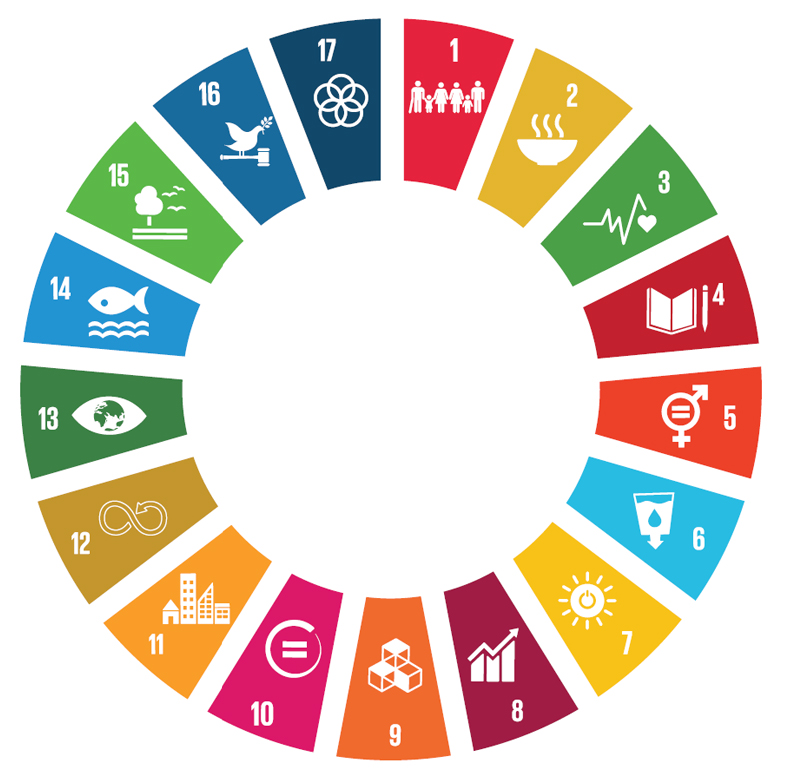
\includegraphics[width=\linewidth]{goals.png}
\caption{\cite{Chora}}
\end{figure}

\begin{document}
\maketitle

\newpage
\begin{titlepage}
\section*{Sammanfattning}
År 2015 kom världens ledare tillsammans med FN överens om en ny handlingsplan för hållbar utveckling. Agenda 2030: Globala mål för hållbar utveckling tar vid där Millenniemålen slutade och bygger på lärdommar från tidigare år. Förhoppningarna på Agenda 2030 är höga och alla FN:s medlemsländer har skrivit på överenskommelsen. Men det finns kritik mot Agenda 2030. Dessa inefattar att målen inte är tillräckligt specifika, att det kan behövas ett bredare systemperspektiv för att se hur målen påverkar varandra med tiden och att agendan skulle gynnas av att ha ett övergripande mål med en tydligare framtidsvision. Det är viktigt att komma ihåg att agendan endast är en överenskommelse och inte bindande, vilket gör att den kan ses som ett opålitlig verktyg för att nå målen. Men trots att det finns ett flertal förbättringsmöjliheter ses Agenda 2030 som ett stort steg framåt i arbetet för en global hållbar utveckling. Att alla länder gemensamt har kommit fram till en handlingsplan trots de många olika åskter och synsätt som skiljer oss åt ger hopp om att denna agenda ska leda världen mot en hållbarare framtid. Den belyser problemen som finns och skapar en viktig dialog och ett utrymme för länder att samarbeta för att skapa den framtid vi vill leva i tillsammans. 

\newpage
\tableofcontents
\end{titlepage}
\newpage
\pagenumbering{arabic}
\section{Inledning}
\subsection{Bakgrund}
Under de senaste århundraderna har människan utvecklats i en takt aldrig tidigare skådad. Detta har bland annat gett upphov till klimatförändringar, utarmade ekosystem, fattigdom och ökande klyftor mellan rika och fattiga länder.\cite{webWWF} Idag räcker det inte längre med att utveckas, för en bättre framtid krävs utveckling på ett hållbart sätt. Hållbar utveckling definieras som utveckling som tillgodoser dagens behov utan att äventyra kommande generationers möjlighter att tillgodose sina behov.\cite{web2030agenda}
För att driva utvecklingen framåt på ett hållbart sätt för världens u-länder enades FN:s medlemsländer år 2000 om Millenniemålen, som behandlar de viktiga punkterna för hållbarhet och utveckling.  Sedan Millenniemålen skapades år 2000 har stora framsteg gjorts i fattigdomsbekämpning, jämställdhet och utveckling. Men det finns mycket kvar att jobba på. \cite{webEuropeanComission}
Agenda 2030: Globala mål för hållbar utveckling är en ny global utvecklingsagenda framtagen av FN och antagen av världens stats- och regeringschefer som tar vid där Millenniemålen slutade år 2015. Denna agenda går djupare in på problemen än vad Millenniemålen gjorde. Den fokuserar på hållbar utveckling i alla länder, inte bara u-länder och erkänner arbete mot klimatpåverkan som en grund för att nå en hållbar utveckling. Men kommer denna agenda att lyckas leda världen mot en hållbarare framtid? Världens ledare har uttryckt höga förhoppningar för denna utvecklingsplan som bygger på erfarenheter från Millenniemålen, men kommer den att leda till resultat?

\subsection{Syfte}
Syftet med denna rapport är att undersöka hur Agenda 2030: Globala mål för hållbar utveckling fungerar som verktyg för att nå den hållbara utveckling som beskrivs i agendan. Vilka förbättringsmöjligheter finns och vad är det som talar för att agendan kommer lyckas med sitt mål? Eftersom Agenda 2030 bygger vidare på Millenniemålen är det även intressant att se vilka lärdomar som har tagits från tidigare år.

\subsection{Metod och källkritik}
Denna rapport är sammanställd genom litteraturstudier. Den huvudsakliga källan är FN men även källor fristående från FN har använts. Försök har gjorts till att inkludera flera olikal synvinklar på Agenda 2030 i denna Rapport. Mycket av faktan har tagits från FN:s hemsida och kan därför vara partisk. Dock så har andra åsikter om agendan inkluderats från källor bedömda som pålitliga. FN anses som en säker källa då det kommer till fakta om agendan och dess utveckling och mycket av det som kommer från andra källor är åsikter som bedömts vara relevanta och byggda på fakta. 

\newpage 
\section{Resultat}
\subsection{Vad är Agenda 2030: Globala mål för hållbar utveckling?}
Agenda 2030 är en ny global utvecklingsagenda från FN som består av 17 globala mål för hållbar utveckling. \cite{webUNASweden} \href{https://sustainabledevelopment.un.org/content/documents/21252030%20Agenda%20for%20Sustainable%20Development%20web.pdf}{Agendan} är en handlingsplan för människorna, planetens och vårt välstånd. De Globala målen tar vid där Millenniemålen slutade och består av 169 delmål för en bättre framtid. I september 2015 hos FN i New York skrev samtliga av FN:s 193 medlemsstater på Agenda 2030 och de Globala målen för hållbar utveckling.\cite{webUNASweden} Målen är universella och gäller både höginkomst- och låginkomstländer \cite{webUNDP}. De Globala målen ska leda världen mot en fredlig och hållbar utveckling till år 2030 och integrerar de tre dimensionerna av hållbar utveckling: social, ekonomisk och miljömässig. \ref{dimensioner}. \cite{webUNASweden}\\

 De 17 globala mål som antagits är: 
\begin{enumerate}
\item Utrota fattigdom i alla dess former, överallt.
\item Utrota hunger, uppnå matsäkerhet och förbättrad kost samt främja ett hållbart jordbruk.
\item Säkerställa hälsosamma liv och främja välbefinnande för alla i alla åldrar.
\item Säkerställa inkluderande och rättvis utbildning av god kvalitet och främja livslångt lärande för alla.
\item Uppnå jämställdhet och stärka alla kvinnors och flickors ställning.
\item Säkerställa tillgänglighet och hållbar förvaltning av vatten och sanitet för alla.
\item Säkerställa tillgång till prisvärd, pålitlig, hållbar och modern energi för alla.
\item Främja kontinuerlig, inkluderande och hållbar ekonomisk tillväxt, full och produktiv sysselsättning och anständigt arbete för alla.
\item Bygga motståndskraftig infrastruktur, främja inkluderande och hållbar industrialisering och främja innovation.
\item Minska ojämlikhet inom och mellan länder.
\item Gör städer och boplatser inkluderande, säkra, flexibla och hållbara.
\item Säkerställa hållbara konsumtions- och produktionsmönster.
\item Vidta brådskande åtgärder för att bekämpa klimatförändringarna och dess effekter.
\item Bevara och hållbart nyttja hav, sjöar och marina resurser för hållbar utveckling.
\item Hållbart skogsbruk, stoppa ökenspridning, bromsa och vända markförstöring samt hejda förlusten av biologisk mångfald.
\item Främja fredliga och inkluderande samhällen för hållbar utveckling, ge tillgång till rättssystem för alla och bygga effektiva, ansvarstagande och inkluderande institutioner på alla nivåer.
\item Stärka verktyg för genomförande och vitalisera det globala partnerskapet för hållbar utveckling. \cite{webKTH}
\end{enumerate}

\begin{figure}[h]
\label{dimensioner}
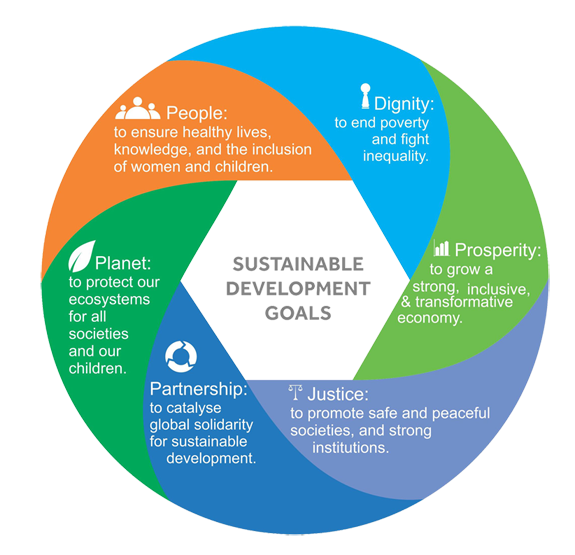
\includegraphics[width=\linewidth]{dimensioner.png}
\caption{De olika aspekterna inkluderade i de Globala målen. \cite{Dochas}} 
\end{figure}

\subsection{Hur ska Agenda 2030 implementeras?} 
Implementering av de Globala målen och dess framgång kommer att bero på ländernas egna policys, planer och program för utveckling. De Globala målen ska fungera som en riktlinje för att styra ländernas planer mot det som överenskommits i Agenda 2030. \cite{web2030agenda}
I Sverige har Sida fått i uppdrag av regeringen att utveckla nya innovativa former för utvecklingsfinansiering. \cite{webSIDA}
Nationellt ledda utvecklingsstrategier kommer att kräva mobilisering av resurser och strategier för finansiering. Regeringen, civilsamhället, den privata sektorn och alla andra förväntas samarbeta för att nå de Globala målen. Men även en global gemenskap kommer krävas för att stödja nationella arbeten.\cite{web2030agenda}\\

\subsection{Vem ansvarar för att Agenda 2030 följs?} 
De Globala målen är inte på något sätt bindande. Länder förväntas själva sätta upp en strategi för att nå de 17 globala målen och implementering kommer att hänga på ländernas egna policies och program för hållbar utveckling. Länderna har själva det huvudsakliga ansvaret att följa upp arbetet. Det finns inget som straffar länder som inte gör sin del för att uppnå de Globala målen som undertecknats i Agenda 2030, eftersom agendan är en överenskommelse mellan länder och inte rättsligt bindande. \cite{web2030agenda}\\

\subsection{Hur ska arbetet finansieras?} 
Att förverkliga dessa mål kommer att kräva stora finansiella insatser och  investering i både u- och i-länder. \cite{web2030agenda}
Hur målen ska implementeras och hur finansiella resurser ska mobiliseras ligger till grund för den nya agendan. \cite{webUNASweden}
Kostnaden beräknas uppgå till triljontals USD, \cite{web2030agenda} ca 4500 miljoner USD per år. Detta är trettio gånger mer än det totala årliga biståndet i världen idag. \cite{webUNICEF} FN:s medlemsländer enades under mötet i New York om ett 100-tal insatser för att finansiera Agenda 2030. Även teknologiöverföring, handel och betydelsen av relevant och bra statistik diskuterades som medel för att uppnå målen. \cite{webUNASweden}
Enligt FN måste resurser mobiliseras från både den kommunala och den privata sektorn, nationellt och internationellt. Det kommer inte att räcka med traditionellt bistånd. Resurserna finns redan i världen men hur investeringar riktas för att stödja hållbar utveckling kommer att spela stor betydelse. Utvecklingshjälp kommer fortfarande att krävas för att hjälpa fattigare länder att nå målen. 
\cite{web2030agenda}
I juli 2015 samlades delegater från hela världen vid FN:s konferens om utvecklingsfinansiering i Addis Abeba. Resultatet blev Addis Ababa Action Agenda, som fastställer hur de Globala målen ska finansieras.\cite{webSIDA}
I agendan kom länderna överens en mängd åtgärder för att finansiera de Globala målen såsom förbättrad skatteinsamling och åtgärder mot taxsmitning. Samarbete och officiell utvecklingshjälp mellan länder, speciellt u-länder, var en annan överenskommelse. Agendan understryker även hur viktigt det är med privat investering och incitament från regeringen för att leda dessa investeringar mot hållbar utveckling. Ett nytt sätt att finansiera ny teknologi till u-länder var också med i överenskommelsen. Den innefattade även internationellt samarbete för finansiering av områden där investering krävs såsom infrastruktur för energi, transport och vatten för att nå de Globala målen.  
\cite{webUNDESA}\\

\subsection{Hur sker uppföljningen och övervakningen av arbetet?} 
Uppföljning och övervakning av målen och arbetet som görs kommer att ske både på global och nationell nivå. Globalt så kommer målen från den nya agendan att mätas mot ett antal globala indikatorer. Dessa indikatorer togs fram av The Inter-Agency and Expert Group on SDG Indicators (IAEG-SDGs) och slogs igenom i mars 2016. \cite{web2030agenda}
Det finns idag en \href{https://unstats.un.org/sdgs/indicators/indicators-list/}{lista} med 232 indikatorer som följs. \cite{webUN2}.
Regeringar kommer också själva att utveckla nationella indikatorer för att hjälpa till att övervaka framstegen som görs för att nå de 17 målen. Det ska resultera i 2 indikatorer för varje delmål. Uppföljningen av dessa mål kommer att samlas i en rapport för FN:s generalsekreterare. De årliga mötena av  “High-level Political Forum on sustainable development” kommer att spela en central roll i utvärderingen av de Globala målen på global nivå. Implementeringsmetoderna kommer att ses igenom för att försäkra att finansiella resurser är mobiliserade på ett effektivt sätt för att nå de Globala målen.  \cite{web2030agenda}\\

\subsection{Vad är skillnaden mellan Millenniemålen och de Globala målen i Agenda 2030?} 
De Globala målen är en fortsättning på Millenniemålen som utgick år 2015. Millenniemålen har hjälpt till att väcka uppmärksamhet till mängder av problem i världen. Sedan Millenniemålen sattes har världens fattigdom halverats, 90 procent av barn i u-länder får nu grundläggande utbildning och jämställdheten har ökat. Det finns dock mycket kvar att jobba på. \cite{webEuropeanComission}
Sedan 1990 har utsläppen av växthusgaser ökat med nästan 50 procent och de fortsätter att öka. Nivån växthusgaser i atmosfären är idag högre än den någonsin varit. \cite{webUN1}
I FN:s utvärdering av millenimålen "The Millennium Development Goals report 2015"  \cite{Millennium} visas det att alla länder med tydliga mål, strategier och politisk vilja kan göra framsteg mot en bättre värld. Rapporten skriver också att dessa framsteg har varit ojämna och fallit kort i flera områden och inte nått många av världens fattigaste och mest utsatta. I rapporten fastslogs att specialinriktade insatser behövs för att nå världens mest utsatta.  Millenniemålen har även visat hur viktigt det är att följa upp målen med data för att uppnå den hållbara utveckling som behövs. Detta är något som de Globala målen bygger vidare på \cite{Millennium}\\

Agenda 2030 bygger på erfarenhet från Millenniemålen för att fortsätta jobba mot en hållbar utveckling. \cite{webEuropeanComission}
De Globala målen är mer omfattande än Millenniemålen var och adresserar problemen på djupet på ett sätt som ska vara hållbart för alla världens länder. De Globala målen är just globala till skillnad från Millenniemålen som i huvudsak var riktade mot u-länder. En viktig del av de Globala målen är att de fokuserar extra mycket på hur de ska implementeras och förverkligas. De nya Globala målen erkänner även att arbete mot klimatförändring är viktigt för hållbar utveckling och bekämpning av fattigdom. \cite{web2030agenda}
Problemen med Millenniemålen har varit att framstegen ofta inte når världens mest utsatta människor såsom de fattigaste och de som lever i konfliktzoner samt de som diskrimineras på grund av kön, ålder, funktionshinder eller etnicitet. Utvecklingen skiljer sig åt mycket mellan länder och trots framsteg finns det mycket kvar att förbättra.\cite{Millennium}\\

\subsection{Vad finns det för kritik mot Agenda 2030?} 
Trots de höga förhoppningarna från världens ledare som skrivit på Agenda 2030 så finns det kritik. Thomas Pogge från Yales Philosophy Department listar upp flera punkter där de Globala målen brister: 

\begin{enumerate}
\item De Globala målen främjar en falsk känsla av framgång och gör det lätt för regeringar att ta det långsamt med att förverkliga de mänskliga rättigheterna. 
\item De Globala målen misslyckas med att specificera vad ett mänskligt rättighetsbaseradt mål för att utrota fattigdom kräver, en tydlig arbetsfördelning. 
\item Ett fullständigt förverkligande av de mänskliga rättigheterna kräver en omfattande förbättring av internationella och nationella jämlikheter, vilket de Globala målen inte kräver. \cite{critique}\\
\end{enumerate} 

Även ICSU och ISSU har satt ihop en rapport där de utvärderar de Globala målen utifrån ett vetenskapligt perspektiv. De skriver i sin rapport att de Globala målen är en betydlig förbättring av Millenniemålen.  De tar upp några av de systematiska hindren som finns för en hållbar utveckling och erbjuder en bättre balans av de tre dimensionerna av hållbar utveckling: social, ekonomisk och miljömässig. De tar även hänsyn till viktiga faktorer såsom ojämlikhet, ohållbar konsumtion, institutionskapacitet och miljöproblem som Millenniemålen utelämnade. Miljömässig hållbarhet är något som lades till senare i Millenniemålen och spelade inte en lika grundläggande roll som det nu gör i de Globala målen. Millenniemålen fokuserade endast på u-länder och fångade bara till en viss del de tre dimensionerna av hållbarhet. En viktig skillnad med de Globala målen är att de ser att alla världens länder behöver sträva efter för en hållbar utveckling, även om olika mål är olika viktiga för alla länder. Trots alla dessa framsteg finns det förbättringar som skulle kunna göras i Agenda 2030. Enligt ICSU och ISSU utvärdering av delmålen är 49st (29 procent) väl utvecklade, 91st (54 procent) skulle behöva vara mer specifika och 29st (17 procent) kräver betydligt mer arbete. Se figur \ref{fig1}. 
I sin rapport \href{http://www.icsu.org/publications/reports-and-reviews/review-of-targets-for-the-sustainable-development-goals-the-science-perspective-2015/SDG-Report.pdf}{"Review of targets for the sustainable development goals: The science perspective"} listar de upp fem punkter med potential för förbättring:  

\begin{enumerate} \label{forbattring}
\item Formulera ett övergripande mål.
\label{improvment1}
\item Utveckla sammanlänkande delmål som är gemensamma för olika mål. 
\label{improvment2}
 \item Formulera en lockande framtidsbild av utvecklingenscenariet.
 \label{improvment3} 
\item Förena och paketera målen och dess interaktioner med varandra. \label{improvment4}
\item Specificera delmålen.
\label{improvment5} \cite{review}
\end{enumerate} \\


\begin{figure}[h] \label{fig1}
\label{improvments}
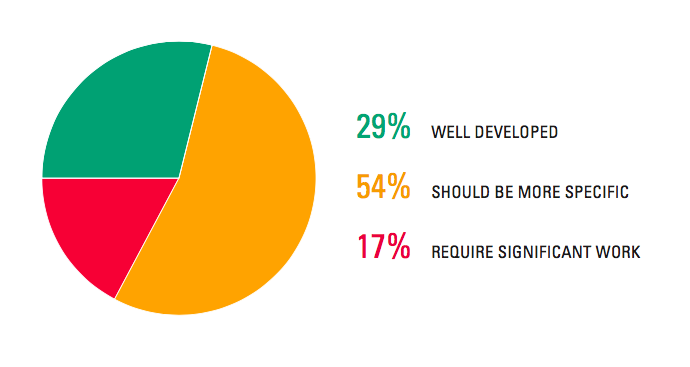
\includegraphics[width=\linewidth]{improvments.png}
\caption{De Globala målen \cite{review}} 
\end{figure}

Förbättringsmöjlighet \ref{improvment1} syftar på att de Globala skulle kunna gynnas av ett övergripande mål som binder samman de 17 målen och beskriver hur dessa mål ska komma till nytta för världen och dess invånare. Även viktiga avvägningar och komplementeringar som rör målen skulle kunna gynnas av att specificeras i ett uppföljningsdokument. ICSU och ISSU har som exempel “A prosperous, high quality of life that is equitably shared and sustainable.”. Detta övergripande mål skulle också kunna hjälpa till att göra agendan mer tillgänglig och förståelig för en större mängd människor.\cite{webC}

Med förbättringsmöjlighet \ref{improvment2} menas att införandet av en målsättning som jobbar från botten och upp och arbetar med funktionellt distinkta enheter kan öka integrationsnivån i målens struktur.\cite{Weitz}
Många av målen påverkar även flera av de andra och arbete för att uppnå ett mål kan ha oönskade effekter på ett annat mål. De flesta målen är integrerade i varandra och ett mål kan påverka ett annat både positivt och negativt. Att istället arbeta för målen på ett integrerat sätt kan bidra till önskade resultat för många av målen. Mål 1 att utrota fattigdom kan exempelvis inte uppnås utan framsteg i mål 2, att uppnå matsäkerhet. Men uppoffringar kommer också att behöva göras. Exempelvis kan en ökning av brukbar mark för att få slut på svält resultera i minskad biodiversitet. Det finns alltså ett behov av att införa ett bredare systemperspektiv som kan beskriva hur målen och delmålen skulle påverka varandra med tiden, på både positiva och negativa sätt, och hur de bidrar till det övergripande målet. \cite{review}\\

Att formulera en lockande framtidsbild av utvecklingenscenariet är en annan förbättringsmöjlighet, punkt \ref{improvment3}. Denna syftar på att det är viktigt att ha en tydlig bild av hur världen skulle se ut om alla målen uppfylldes för att tydligt kunna kommunicera och dela de Globala målen med världen. Denna framtidsbild skulle kunna öka förmågan att hantera svåra avvägningar i utförandet av målen och starta diskussionen om vilken framtid som bör eftersträvas.\cite{webCostanza1}\\

I överenskommelsen Rio+20 står det att de Globala målen ska vara begränsade i antal, koncista och lätta att kommunicera. Att samla målen under större teman är något som skulle kunna förbättra detta enligt punkt \ref{improvment4} och göra det lättare att nå ut med målen till allmänheten. Det kan dock samtidigt vara bra att ha behålla de 17 målen separata då många aktörer och investerare endast är intresserade av vissa specifika mål. \cite{review}\\

Med punkt \ref{improvment5} menas att en del mål saknar fokus för att kunna implementeras effektivt och skulle gynnas av att specificera potentiella tillämpningsområden. Det är viktigt att kunna mäta om tillräckliga framsteg görs och stora analytiska och politiska insatser krävs för att kunna förbättra de Globala målens struktur. Många av miljömålen är exempelvis betydligt otydligare än de sociala målen. Det borde också specificeras vilka aktörer som förväntas rikta in sig på vilka mål och vilka incitament som ska införas för att detta ska ske. Det nuvarande ramverket för de Globala målen identifierar inte heller de olika sociala grupper som kommer att spela en viktig roll för att uppnå målen utöver regeringar och institutioner. \cite{review}\\



\newpage
\section{Diskussion}
De Globala målen bygger på erfarenheter från Millenniemålen och har därför kunnat utvecklas till en ännu starkare agenda än den föregående. Agenda 2030 fokuserar extra mycket på implementering och finansiering, jobbar på att förbättra insamling av data, tar hänsyn till miljöaspekten som en viktig del för en hållbar utveckling och ser att hållbar utveckling inte bara handlar om u-länder utan om hela världen. Att alla FN:s medlemsländer har skrivit på agendan är väldigt positivt. Hållbar utveckling betyder inte nödvändigtvis samma sak för alla. Vad som är viktigast för varje enskilt land beror på många olika faktorer. För en del länder är det allra viktigaste att komma ur fattigdom och att landets invånare får sina dagliga behov, såsom mat för dagen, uppfyllda. Andra länder tycker att det viktigaste är teknikutveckling och byte till förnybara energikällor. Allt beror på de förutsättningar landet har och vad de själva har för problem att överkomma. Att alla dessa länder tillsammans har kommit fram till 17 mål som ska leda mot en hållbarare framtid är otroligt. Det visar att samtliga länder är villiga att ta tag i dagens problem och ser behovet att tillsammans arbeta mot en hållbar framtid. \\

Det är dock viktigt att komma ihåg att de Globala målen är en överenskommelse mellan länder och inte ett rättsligt bindande kontrakt. Detta skapar en möjlighet för länder att fly från sina förpliktelser. Men det skapar även möjlighet för länder att anta en mer ambitiös agenda om så önskas. Detta kan vara ett problem men å andra sidan så har samtliga länder skrivit på agendan vilket visar att de är medvetna om problemet och vill lösa det.  Vi kan se att framsteg har gjorts sedan Millenniemålen implementerades vilket får tron på att denna nya förbättrade agenda ska lyckas, att bli ännu starkare. \\

Världens ledare har uttryckt sig positivt till denna agenda och det finns höga förhoppningar på vad den ska kunna åstadkomma. Det är svårt att säga hur mycket av denna agenda som kommer kunna förverkligas. Det beror på hur världens länder agerar och om de kan samarbeta för att uppnå dessa globala mål. Men om man ser till vad som tidigare åstadkommits med Millenniemålen så ser det positivt ut. Att helt uppfylla alla mål till 2030 känns en aning ambitiöst men att komma en bra bit på vägen känns lovande och möjligtvis är en ambitiös agenda vad som krävs för att få länder att göra allt de kan för en bättre framtid. Att ha tydliga delmål och planer för hur de ska genomföras är dock något som är viktigt för att man ska känna att utvecklingen går åt rätt håll och uppmuntra till fortsatt arbete. Det kan vara lätt att tappa bort sig om man inte har tydligt planerade delmål och detta är något som skulle kunna förbättras i agendan. Sett i jämförelse med Millenniemålen har de Globala målen tydliga delmål och har fokuserat mycket på implementering och finansiering av arbetet men det finns rum för förbättring. Olika delar av målen är även olika specifika. Exempelvis så är många av miljömålen betydligt otydligare än de sociala målen. Detta kan göra det svårt att på ett enhetligt sätt mäta framgången i målen och är något som är mycket viktigt för att kunna förbättra implementering och se till så att arbetet sker på rätt sätt. Av de 8 Millenniemålen skedde det betydande framgång i fattigdomsbekämpning, jämställdhet och utveckling, men utsläppen av växthusgaser fortsatte öka. Övervakningen av Millenniemålen har tydligt visat att insamling av data är en viktig del av arbetet med målen och detta har man tagit lärdom av och försökt förbättra i de nya Globala målen.\cite{Millennium} Eftersom man utvärderat Millenniemålen och kunnat ta vara på dess lärdom när de Globala målen skapades finns det hopp om att dessa ska kunna åstadkomma desto mer. \\

Eftersom länder har olika förutsättningar för att uppnå målen kan det krävas olika mål för olika länder. Länder som kan göra mer borde göra mer och hjälpa de länder som behöver finansiellt stöd för att nå de satta målen. Globalt samarbete är något som understryks i agendan och som förhoppningsvis kan fortsätta förbättras. Detta kräver att länder kan se förbi sina egna gränser eftersom detta är ett världsomfattande problem.
De förbättringsmöjligheter som tas upp i \href{http://www.icsu.org/publications/reports-and-reviews/review-of-targets-for-the-sustainable-development-goals-the-science-perspective-2015/SDG-Report.pdf}{"Review of targets for the sustainable development goals: The science perspective"} är bra och väl genomtänkta förslag till förbättringar hos agendan. Trots brister är det bra att ha en agenda som alla världens FN-medlemmar har kommit överens om. Oavsett hur det går för agendan så känns det som ett stort steg i rätt riktning att alla länder har kommit överens om detta och ser problemen. Om problemen inte tas upp så kommer de heller inte att kunna åtgärdas. De Globala målen har en del brister och eftersom de inte är bindande måste viljan och drivkraften att förändras finnas världen över. Detta kan ses som något osäkert då alla länder har egna agendor och problem som kan komma i vägen för de Globala målen. Samtliga länder har också olika mål inom agendan som är viktiga och mindre viktiga för landets utveckling. Allt detta kan komma att påverka hurvida agendan uppfylls. Men trots osäkerheterna med dessa mål som verktyg för en hållbar utveckling utgör de en viktig del av arbetet mot en hållbar framtid genom att belysa problemen och skapa ett samarbete och en viktig dialog mellan och inom länder. \\



\newpage
\section{Slutsats}
Trots en del svagt formulerade mål och andra förbättringsmöjligheter är Agenda 2030: Globala mål för hållbar utveckling ett stort steg framåt i arbetet för en hållbar framtid. För att uppnå en global hållbar utveckling krävs att samtliga länder är villiga att samarbeta, något som har visats då världens ledare kom överens om Agenda 2030. De Globala målen har utvecklats med erfarenhet från Millenniemålen i ryggen och har resulterat i en starkare och bättre agenda än tidigare.

\bibliographystyle{plain}
\bibliography{references} 



\end{document}
